 % Matthias Text
\subsection{Entscheidungsbaum}
\begin{frame}
\frametitle{Analysemethoden}
\framesubtitle{Entscheidungsbaum}
\begin{itemize}\setlength\parskip{12pt}
\item Teilt in Klassen auf
\item Wahr- oder Falsch-Entscheidungen
\item Jedes Blatt hat genau eine Klasse
\item Verwende \texttt{rpart}
\end{itemize}
\end{frame}

\begin{frame}
\frametitle{Analysemethoden}
\framesubtitle{Entscheidungsbaum}
\begin{center}
	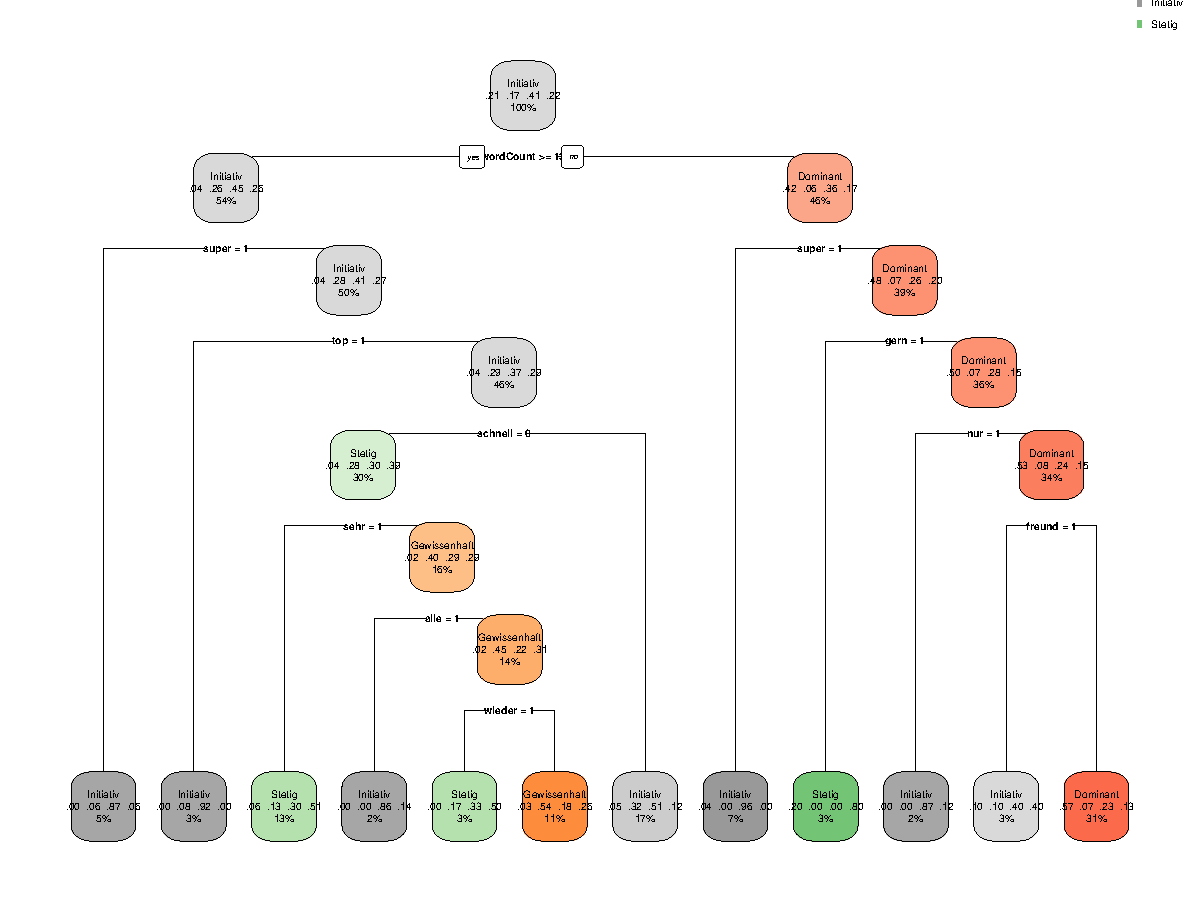
\includegraphics[scale=0.5]{Rplot.pdf}
\end{center}

\end{frame}
%<-------------Folie--------->
\begin{frame}
\frametitle{Analysemethoden}
\framesubtitle{Entscheidungsbaum}
Resultate Entscheidungsbaum, \texttt{R}, Wortaufkommen $> 20$
\begin{center}
\begin{tabular}{|c|c|c|c|c|c|c|c|c|}
\hline
 &  D 	& G	& I & S	& Acc.	& Prec. & Recall	& F1\\
\hline
Dominant & 14 & 3 & 9 & 1 & & 0.518 & 0.777 & 0.621 \\
Gewissenhaft & 0 & 3 & 5 & 5& &0.23 & 0.21,4 & 0.221\\
Initiativ & 2 & 4 & 19 & 5& & 0.633& 0.527 & 0.575\\
Stetig & 2 & 4 & 3 & 7& &0.437 & 0.388& 0.411 \\
\hline
Total 	&		&		& & 		& 0.5	& 0.454& 0.476 & 0.454\\
\hline
\end{tabular}
\end{center}
\end{frame}
%<-------------Folie--------->
\begin{frame}
\frametitle{Analysemethoden}
\framesubtitle{Entscheidungsbaum}
Resultate Entscheidungsbaum, \texttt{Python}, mind. in 1\% der Texte, Englisch
\begin{center}
\begin{tabular}{|c|c|c|c|c|c|c|c|c|}
\hline
 &  D 	& G	& I & S	& Acc.	& Prec. & Recall	& F1\\
\hline
Dominant &     9 & 4 & 12 & 5& &0.3 & 0.5 & 0.375 \\
Gewissenhaft & 2 & 3 & 4 & 2&& 0.272 & 0.214 & 0.239 \\
Initiativ &    5 & 5 & 12 & 8&& 0.4 & 0.333 & 0.363\\
Stetig &       2 & 2 & 8 & 3&& 0.2 & 0.166& 0.181 \\
\hline
Total 	&		&		& &	& 0.313		& 0.293 & 0.303 & 0.289 \\
\hline
\end{tabular}
\end{center}
\end{frame}
%<-------------Folie--------->
\begin{frame}
\frametitle{Analysemethoden}
\framesubtitle{Entscheidungsbaum}
Resultate Entscheidungsbaum, \texttt{Python}, mind. in 1\% der Texte, Deutsch
\begin{center}
\begin{tabular}{|c|c|c|c|c|c|c|c|c|}
\hline
 &  D 	& G	& I & S	& Acc.	& Prec. & Recall	& F1\\
\hline
Dominant &     13 & 4 & 16 & 1&&  0.382 & 0.722 & 0.499 \\
Gewissenhaft & 2 & 4 & 1 & 3 &&  0.4 & 0.285 & 0.332  \\
Initiativ &    3 & 5 & 13 & 7&& 0.464 & 0.361 & 0.406  \\
Stetig &       0 & 1 & 6 & 7 &&  0.5 & 0.388 & 0.436 \\
\hline
Total 	&		&		& & 		&  0.430			&  0.436 &0.439 & 0.418 \\
\hline
\end{tabular}
\end{center}
\end{frame}
%<-------------Folie--------->
\subsection{Random Forest}
\begin{frame}
\frametitle{Analysemethoden}
\framesubtitle{Random Forest}
\begin{itemize}\setlength\parskip{12pt}
\item Entscheidungsbaum nicht beste Option
\begin{itemize}
	\item Gut für Trainingsdaten
	\item Nicht flexibel 
	\item Probleme mit neuen Datensätzen
\end{itemize}
\item Generiere neue Testdaten durch Wählen mit Zurücklegen
\item Erzeuge Entscheidungsbaum
\item Generiere so viele Entscheidungsbäume
\item Entscheidung durch Mehrheitsentscheidung
\item \texttt{R} \texttt{randomForest} 2000 Bäume, analog in  \texttt{Python}
\end{itemize}
\end{frame}
%<-------------Folie--------->
\begin{frame}
\frametitle{Analysemethoden}
\framesubtitle{Random Forest}
Resultate Random Forest, \texttt{R}, Wortaufkommen $> 20$
\begin{center}
\begin{tabular}{|c|c|c|c|c|c|c|c|c|}
\hline
 &  D 	& G	& I & S	& Acc.	& Prec. & Recall	& F1\\
\hline
Dominant & 14 & 2 & 10& 0 &&0.538 & 0.777 & 0.635 \\
Gewissenhaft & 2 & 4 & 0 & 1&&0.571 & 0.285 & 0.28 \\
Initiativ & 2 & 7  & 25 & 14&&0.52 & 0.694 & 0.594 \\
Stetig & 0 & 1 & 1 &  3&&0.6 & 10.66 & 0.26 \\
\hline
Total 	&		&		& & 		& 0.534		&   0.557 & 0.48 & 0.442\\
\hline
\end{tabular}
\end{center}
\end{frame}
%<-------------Folie--------->
\begin{frame}
\frametitle{Analysemethoden}
\framesubtitle{Random Forest}
Resultate Random Forest, \texttt{Python}, mind. in 1\% der Texte, Englisch
\begin{center}
\begin{tabular}{|c|c|c|c|c|c|c|c|c|}
\hline
 &  D 	& G	& I & S	& Acc.	& Prec. & Recall	& F1\\
\hline
Dominant & 16 & 4 & 14 & 4 &&0.421 & 0.888 & 0.571 \\
Gewissenhaft & 0 & 6 & 2 & 1&&0.666 & 0.428 & 0.521 \\
Initiativ & 1 & 4 & 16 & 9&&0.533 & 0.444 & 0.484 \\
Stetig & 1 & 0 & 4 & 4&&0.444 & 0.222 & 0.296 \\
\hline
Total 	&		&		& & 		& 0.488		&  0.516 & 0.495 & 0.468\\
\hline
\end{tabular}
\end{center}
\end{frame}
%<-------------Folie--------->
\begin{frame}
\frametitle{Analysemethoden}
\framesubtitle{Random Forest}
Resultate Random Forest, \texttt{Python}, mind. in 1\% der Texte, Deutsch
\begin{center}
\begin{tabular}{|c|c|c|c|c|c|c|c|c|}
\hline
 &  D 	& G	& I & S	& Acc.	& Prec. & Recall	& F1\\
\hline
Dominant & 15 & 4 & 15 & 2 &&0.416 & 0.833 & 0.554 \\
Gewissenhaft & 0 & 3 & 4 & 3&&0.3 & 0.214 & 0.249 \\
Initiativ & 2 & 4 & 15 & 9&&0.5 &0.416 & 0.454 \\
Stetig & 1 & 3 & 2 & 4&&0.4 & 0.222 & 0.285 \\
\hline
Total 	&		&		& & 		& 0.43		&    0.404 & 0.421 & 0.385\\
\hline
\end{tabular}
\end{center}
\end{frame}
